\subsection{Data statistics and analysis}

In this section we present the quantitative and qualitative analysis of the RedDust resource. In Table \ref{stats_table} we present the overall
statistics of the dataset. Figure \ref{num_posts} shows the chart of the user count per each post count. From this plot we conclude that the users in our dataset tend to have a small number of posts.

\begin{table}[h!]%\sffamily
\centering
\small
\begin{adjustbox}{width=0.55\textwidth}
\begin{tabular}{lrrr}
\toprule
\textbf{attribute} & \textbf{\#users} & \textbf{\#posts} & \textbf{\#subreddits} \\
\midrule
gender & 54.88K & 2.49M & 28.25K \\
age & 122.20K & 5.80M & 44.07K \\
family status & 11.77K & 0.56M & 14.76K \\
profession & 74.86K & 3.63M & 37.49K \\
hobby & 89.07K & 4.42M & 41.31K \\
\midrule
total & 352.78K & 16.9M & 165.88K \\
\bottomrule
\end{tabular}
\end{adjustbox}
\caption{Overall RedDust statistics for each attribute.}
\label{stats_table}
\end{table}

\begin{figure}[!h]
\centering
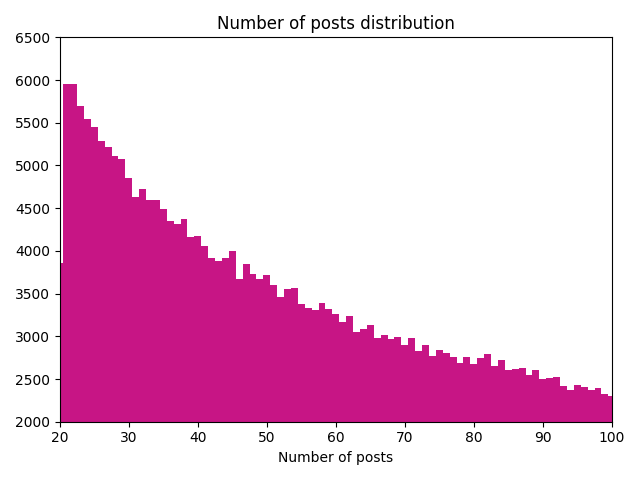
\includegraphics[width=0.55\textwidth]{data/pics/num_posts.png}
%\vspace*{-0.3cm}
\caption{Counts of users having $x$ number of Reddit posts.}
\label{num_posts}
\end{figure}

Almost 19K users in RedDust have two personal attributes known, 980 users have three and 28 have four attributes known,
which amounts to 6\% of the users having multiple personal attributes in total.
For  
such users
it is interesting to look at the interplay between different personal traits, for instance, the correlation between users' occupations and general interests.
In Figure \ref{prof-hob} we plot a heat map which represents the co-occurring values for these two predicates. 
For this experiment as well as the subsequent ones, we limit the number of professions and hobbies to the top $k$ ones ($k=20$ and $k=30$ for \textit{profession} and \textit{hobby}, respectively), sorted by the number of labeled users per value.

We observed intuitive correlations such as:
\emph{musicians} often play \emph{guitar};
\emph{runners} have \emph{running} as the main interest; 
\emph{college students} like to \emph{read} but are also interested in \emph{video games} five times as much as any other professions;
and curiously, \emph{shooting} is popular among \emph{photographers}, most probably because of \textit{shooting} being an ambiguous term.

\begin{figure*}[]
  \centering
  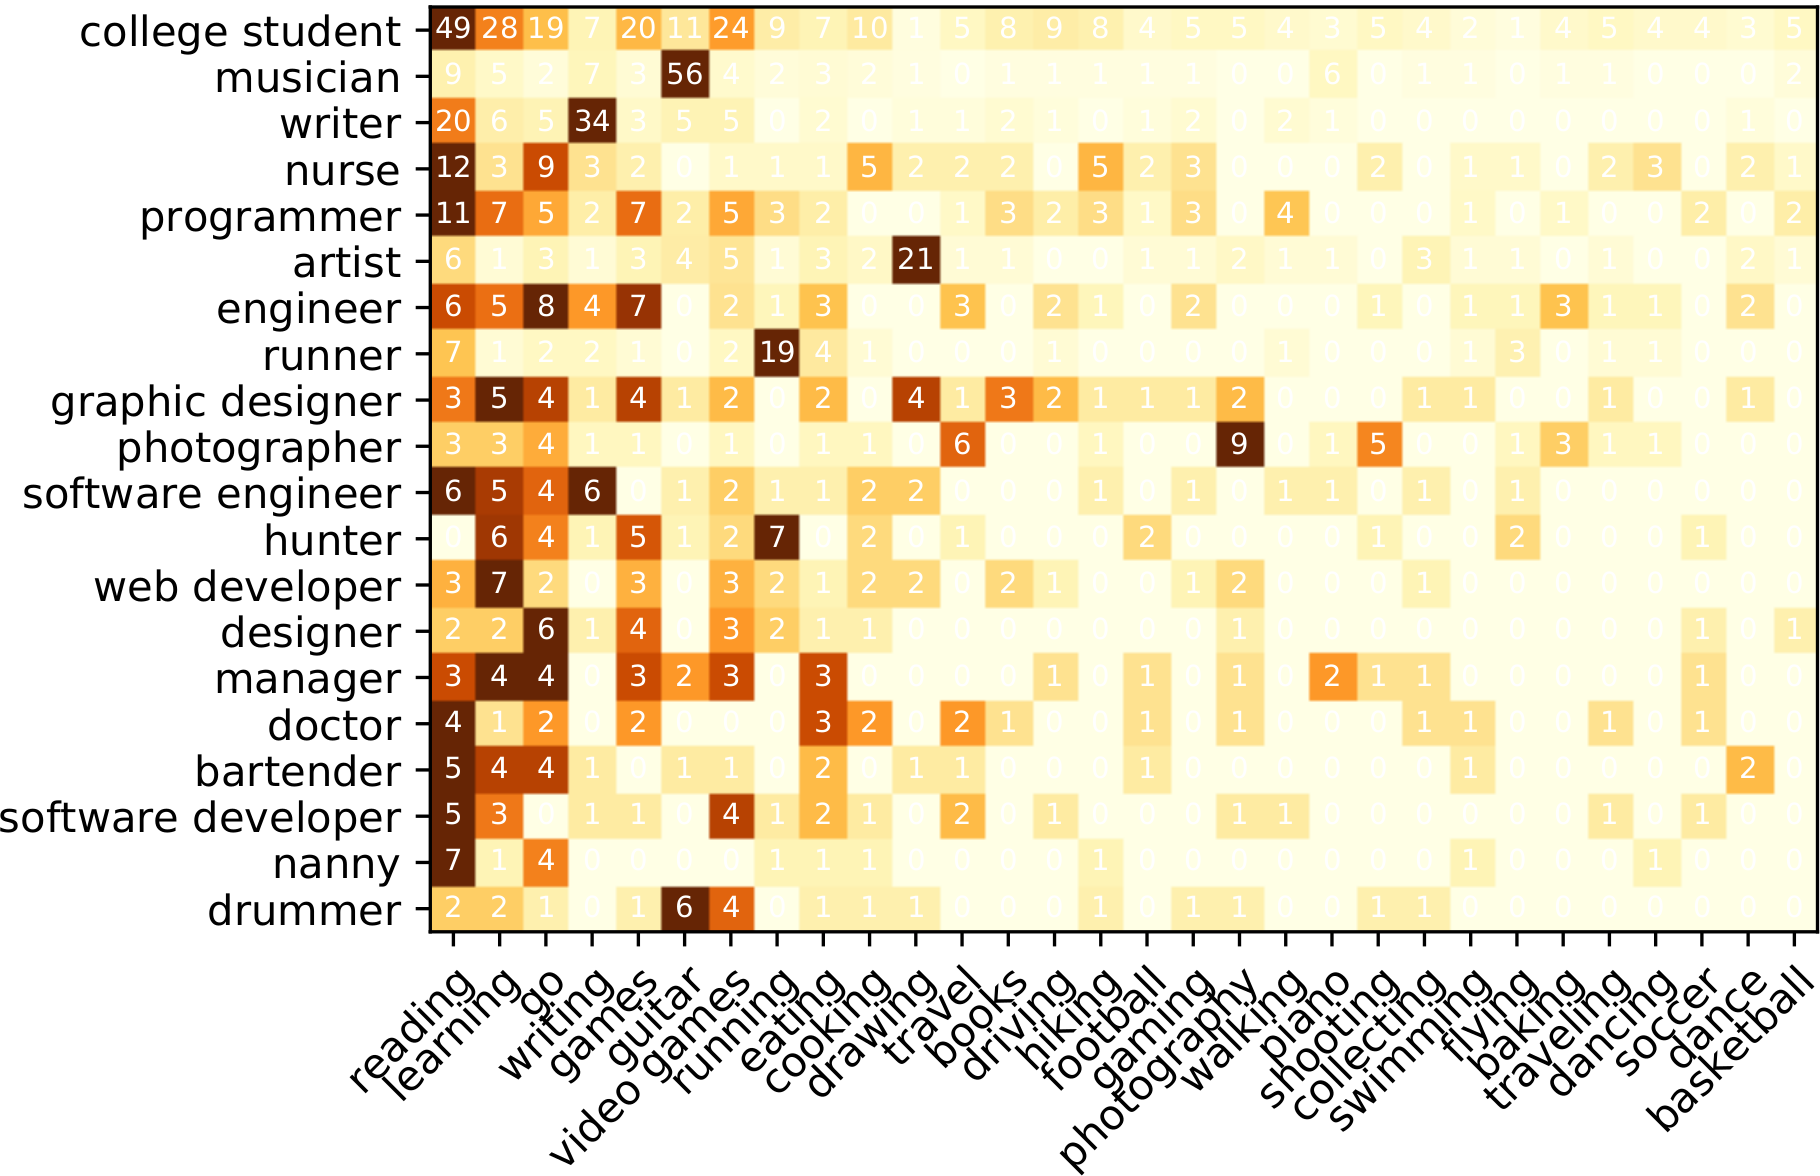
\includegraphics[width=0.77\linewidth]{data/pics/hob_prof.png}
  \caption{Co-occurrence of the most common professions and hobbies.}
  \label{prof-hob}
\end{figure*}

We also considered other pairs of attributes, namely \textit{profession} and \textit{gender}, for which we show the gender distribution of each profession in Figure \ref{prof_gender}. 
The analysis revealed common prejudices like \emph{female nannies} or \emph{male programmers},  
as well as several surprising insights (prevalence of \textit{female runners} and \textit{bartenders}) possibly specific to Reddit communities.

\begin{figure*}[]
\centering
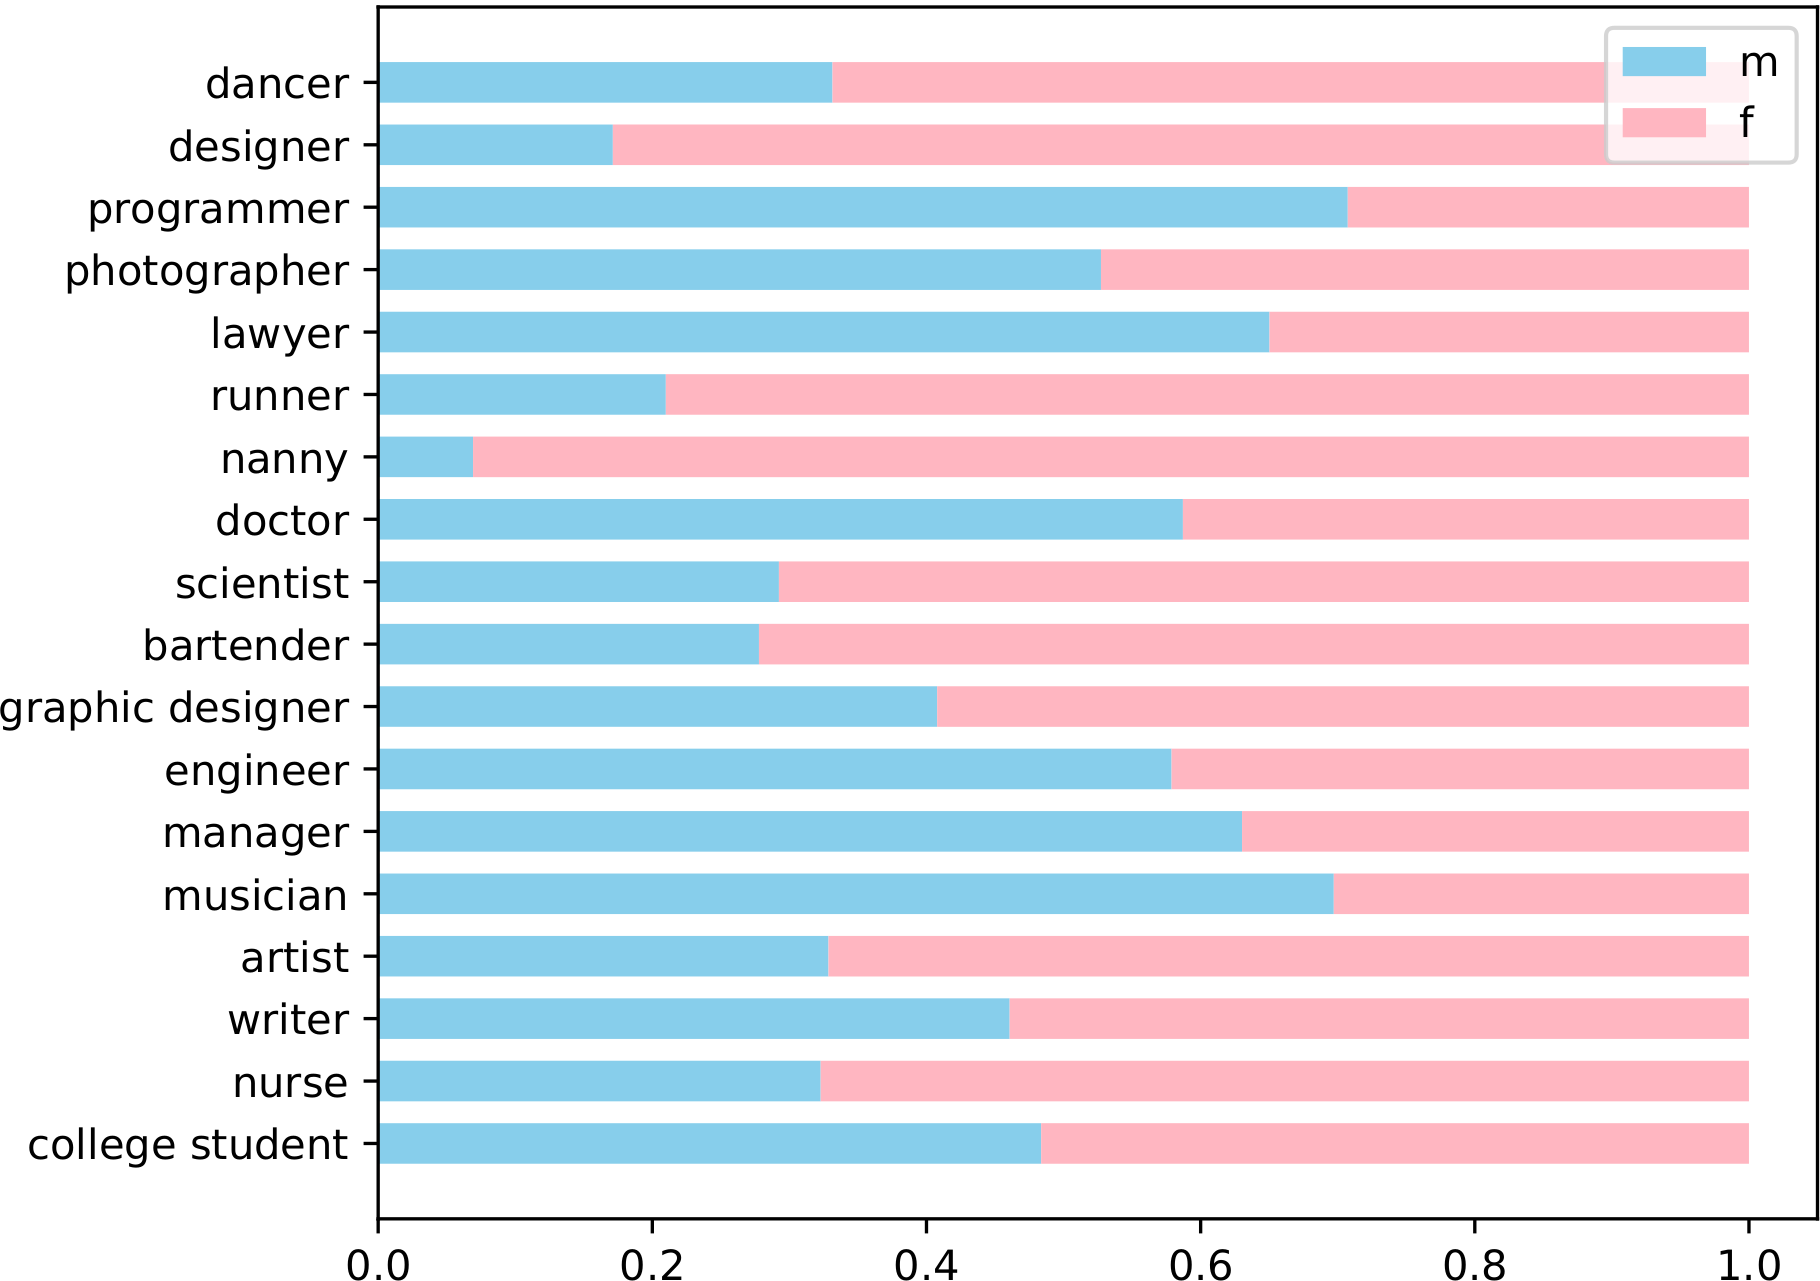
\includegraphics[width=0.67\linewidth]{data/pics/prof_gend.png}
\caption{Gender distribution among professions.}
\label{prof_gender}
\end{figure*}